\mainsection{4}{Dense Neural Networks}{15/05/2020}

\section{Activation function}
Mild requirements on $ \phi() $: \\
\textbullet nonlinear in general $ \rightarrow $ fundamental \\
\textbullet smooth, differentiable $ \rightarrow $ for training \\
\textbullet simple calculation $ \rightarrow $ low complexity \\
\textbullet Slides 4-6; 4-7 activation function types \\

\subsection{Sigmoid activation function}
$ \phi (a) = \sigma (a) = \dfrac{1}{1 + e^{-a}} $ \\
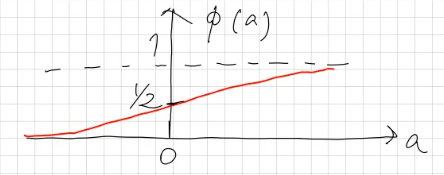
\includegraphics[width=\linewidth]{Images/SigmoidActivationSketch.png}\\
\textbullet $  0 < \phi < 1 \overset {\hat{}}{=}  $ prob.\\
\textbullet symmetry: $ \phi(-a) = 1-\phi(a)  $ \\
\textbullet derivative: $ \dfrac{d \phi(a) }{da} = ... = \dfrac{e^{-a}}{(1+ e^{-a})^2}  = \phi (a) \cdot \phi (-a ) = \phi (a) (1- \phi (a) ), \in (0,1) $\\
easy calculative \\
\textbullet widely used in conventional NN (shallow) \\
\subsection{hyperbolic tangent activation function }
$ \phi (a) = tanh(a) = \dfrac{e^{a} -e^{-a}  }{e^{a}  + e^{-a} }    $ \\
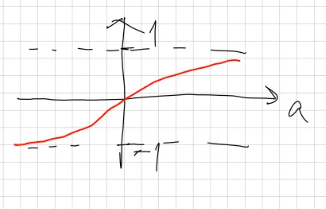
\includegraphics[width=\linewidth]{Images/HyperbolicTangentActivation.png} \\
 like sigmoid but another output range 
 \subsection{rectifier linear unit(ReLU}
 $  \phi (a ) = ReLU(a) = max (a,0) =  \left\lbrace \begin{array}{lc}
 a & a \geq 0 \\
 0 & a < 0 
 \end{array} \right.$ \\
 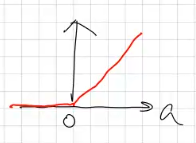
\includegraphics[width=\linewidth]{Images/ReLuActivation.png}\\
 \textbullet $ \equiv $ diode \\
 simple calculation \\
 \textbullet $  \dfrac{d \phi}{da} = \left\lbrace \begin{array}{lc}
 1 & a > 0 \\
 0 & a <0 
 \end{array} \right.  = u(a), u(0) = 0$ typically used \\
 \textbullet most popular in DNN \\
 \textbullet Details on 4-7
 \subsection{Softmax activatoin function(classification problem)}
 $  \phi (\underline{a} : \underline{a}  = [a_i ] \in \Re^c \rightarrow \Re^c$ \\
 $  \phi ( \underline{a}) = softmax (\underline{a}) = \left[
 \begin{matrix} 
\  \phi_1 (\underline{a}) \\
  \vdots \\
  \phi_c (\underline{a})
 \end{matrix} \right] $ \\
 $ \phi (\underline{a}) = \dfrac{ a^{a_i}}{\sum_{j=1}^{c} e^{a_i }} , \in (0,1) , \sum_{i=1}^{c} \phi_i (\underline{a}) = 1 $ \\
 \textbullet maps $  \underline{a} \in \Re^c  $ to a categorical PMF with $ c $ classes  \\
 \textbullet $  a_i  $ large$  \rightarrow \phi_i (\underline{a} )  $ close to 1 \\
 \textbullet $  a_i  $ small $ \rightarrow \phi_i (\underline{a} )  $ close to 0 \\
 \textbullet used in the output layer for classification problems \\
 \section{Special case c=2, binary classification problem}:
 $ \phi_1 (\underline{a}) = \dfrac{e^{a_i}}{e^{a_1} + e^{a_2}} = \dfrac{1}{1+ e^{-(a_1 - a_2)}} = \sigma (a_1 - a _ 2) \\
 \phi_2 (\underline{a} = \dfrac{e^{a_2}}{e^{a_1} + e^{a_2}} = 1 - \phi_1 (\underline{a}) = \sigma (a_2 - a_1) \\
 $
 i.e. softmax \\
 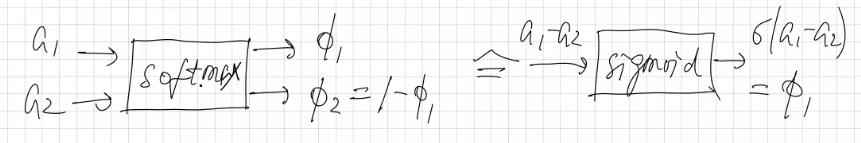
\includegraphics[width=\linewidth]{Images/OutputLayerSoftmax.png} \\
  one sigmoid output is sufficient for binary classification instead of 2 output softmax! \\
\textbf{  Derivative of softmax:}\\
  $ \dfrac{ \partial \phi_i (\underline{a}) }{\partial a_j} = ... = \left\lbrace \begin{array}{lc}
\phi:i (\underline{a})\cdot ( 1- \phi_i (\underline{a}) & i=j \\
- phi_i (\underline{a}) \cdot \phi_j (\underline{a}) & i \neq j 
  \end{array} \right. $
  \textbullet 4-9 for details on usage \\
  \section{Chapter 4.5 Universal approximation } 
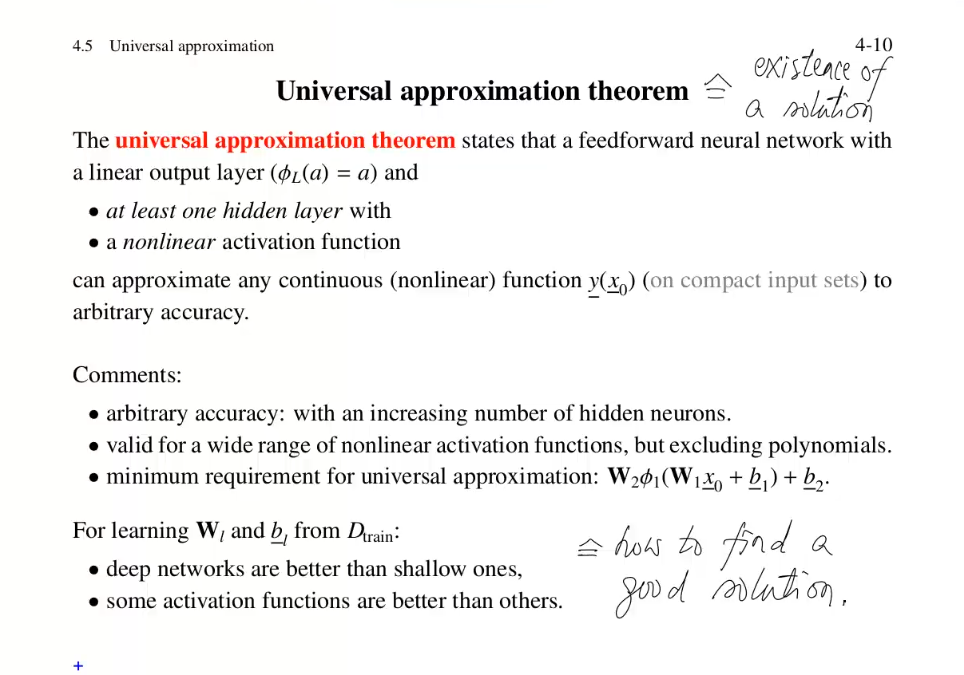
\includegraphics[width=\linewidth]{Images/Slide410.png}

\subsection{E4.3 Regression with 1 hidden layer}
True function: $ f_0(x)   $\\
Given: $ x(n)  $ and noisy function $ y(n) = f_(x(n)) + z(n) , 1 \leq n \leq N  ,z(n)$ is the noise \\
NN: \\
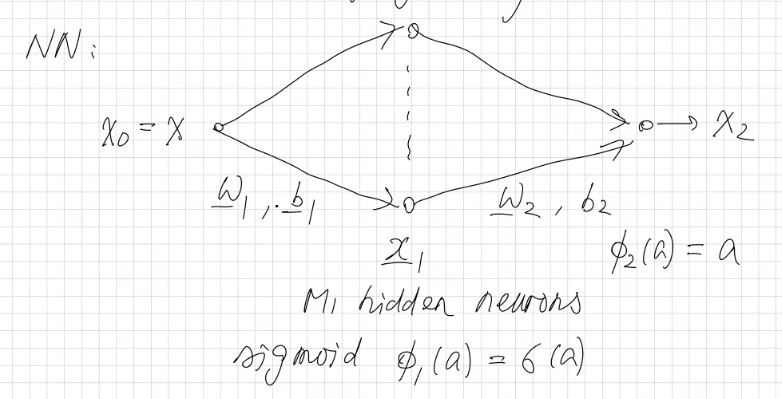
\includegraphics[width=\linewidth]{Images/E43Architecture.png}\\
i.e. $  x_2 = f(x, \underline{\theta}) = \underline{w}_2^T \sigma ( \underline{w}_1 x + \underline{b}_1 )  $, column times row times scalar \\
$ = \sum_{i=1}^{N_1} w_{2,i} \cdot \underbrace{\sigma ( w_{1,i} x + b_{1,i}) }_{M_1 \text{ nonllinear basis functions of }x} + b_2$ \\
$ \sigma ( w_i x + b_i ) \sigma (w_i ( x + \dfrac{b_i}{w_i})) $ \\
new center at $ \dfrac{-b_i}{w_i} $ and new slope value $ w_i $ \\
Picture is for black 1 $ w_i $ red another $ w_i $ green another example $ w_i $\\
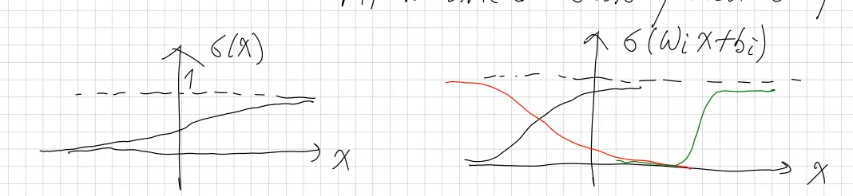
\includegraphics[width=\linewidth]{Images/E43Sketchsigmoid.png}
\section{Chapter 4.4 - 4.6 Loss and cost function}
\textbf{Review chapter 3.4}	\\
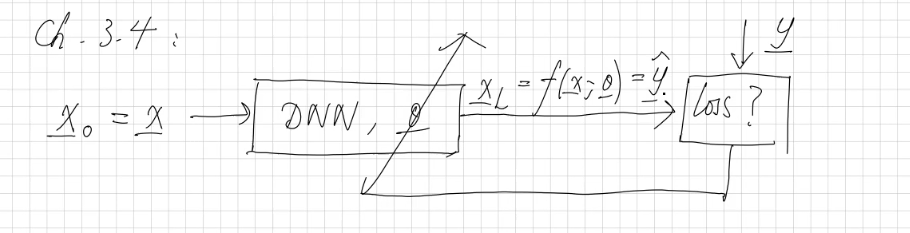
\includegraphics[width=\linewidth]{Images/ProbabalisticFrameworkSupervisedLearning.png}\\
$ \underset{\underline{\theta}}{min}  L ( \underline{\theta  }) =  \dfrac{1}{N} = \sum_{n=1}^{N} (l(\underline{x}(n), y(n)_i \underline{\theta}$     cost dunction for $ d_{train } $ \\
$l(\underline{x}, \underline{y}_j \underline{\theta }) = - ln(q ( \underline{y} | \underline{x}_j \underline{\theta } )  $ loss for one pair $  (\underline{x}, \underline{y})  $ \\
$  q () \leftrightarrow $ DNN ???\\


	
	
	
	
	
	
	
	
	
	
	
	
	
	
	
	
	
	
	
	
	
	
	
	
	
	
	
	
	
	
	
	
	
	
	
	
	
	
	
	
	
	
	
	
	